% Standalone TikZ source for the Glaukopis chained-IFT process diagram.
% Compile with: pdflatex glaukopis_chained_ift.tex
% Renders to PNG with: pdftoppm -r 300 glaukopis_chained_ift.pdf glaukopis_chained_ift -png
\documentclass[tikz,border=6pt]{standalone}
\usepackage[T1]{fontenc}
\usetikzlibrary{arrows.meta,positioning,fit,backgrounds,calc,shapes.geometric}

\begin{document}
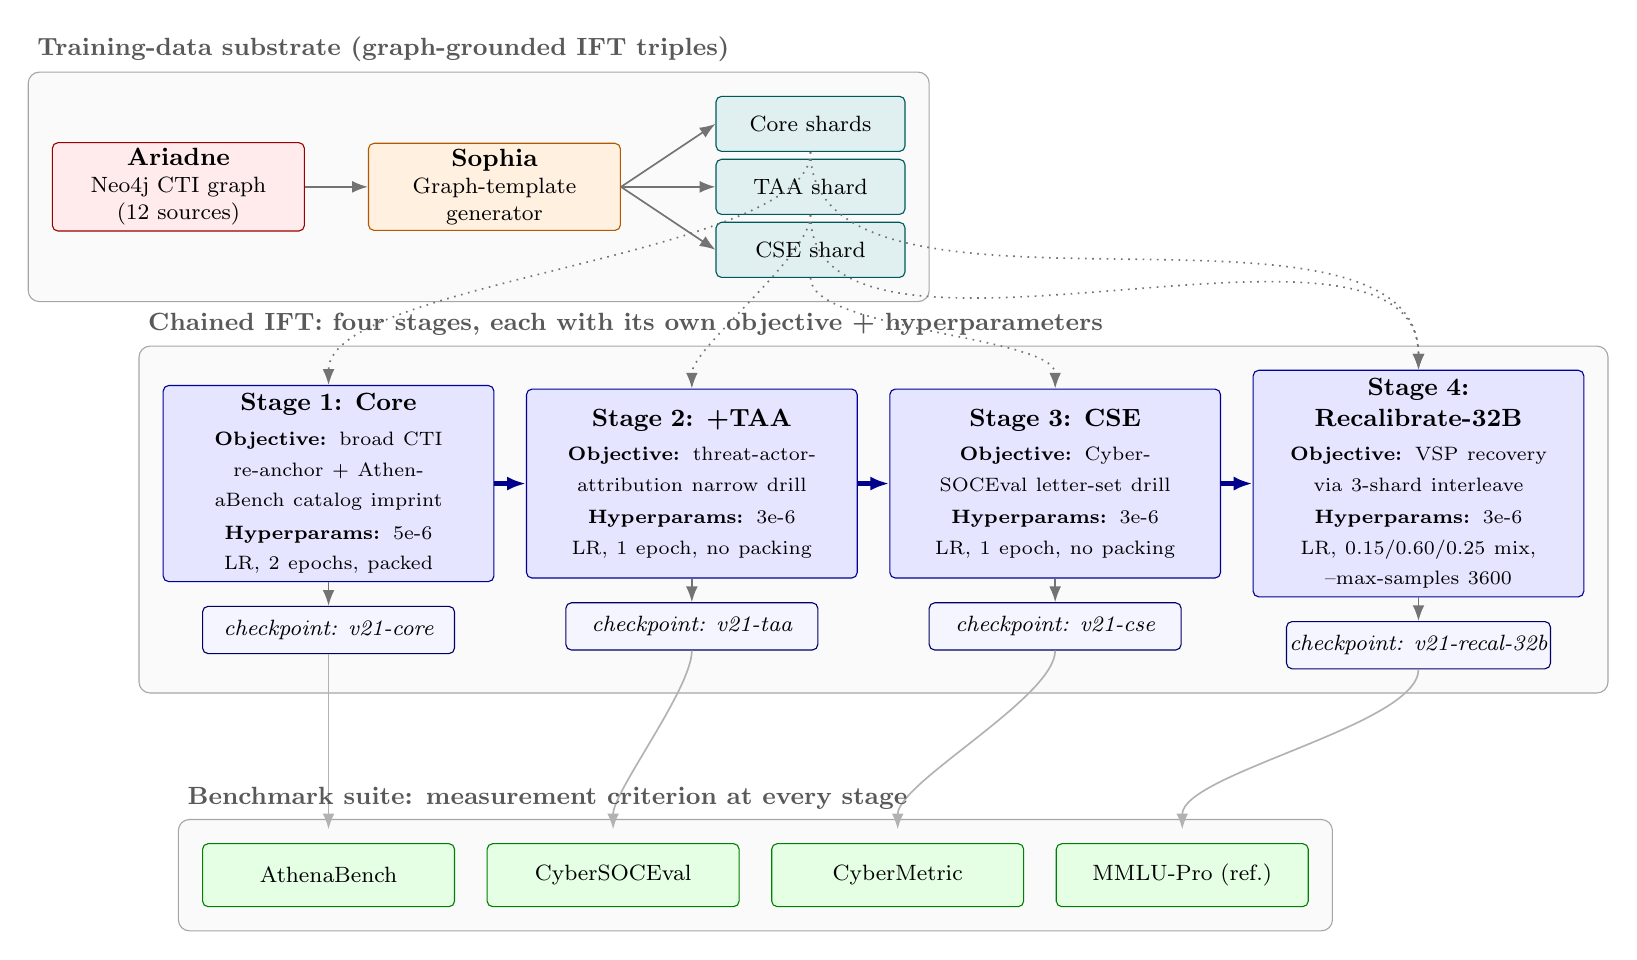
\begin{tikzpicture}[
    font=\rmfamily\small,
    >={Latex[length=2.2mm]},
    node distance=4mm and 6mm,
    src/.style       ={rectangle, rounded corners=2pt, draw=red!60!black, fill=red!8,
                       minimum width=32mm, minimum height=10mm, align=center, inner sep=2pt},
    shard/.style     ={rectangle, rounded corners=2pt, draw=teal!70!black, fill=teal!12,
                       minimum width=24mm, minimum height=7mm, align=center, inner sep=2pt,
                       font=\rmfamily\footnotesize},
    stage/.style     ={rectangle, rounded corners=2pt, draw=blue!60!black, fill=blue!10,
                       minimum width=42mm, minimum height=24mm, align=center, inner sep=3pt,
                       text width=39mm},
    obj/.style       ={font=\rmfamily\scriptsize, align=left, text width=37mm},
    ck/.style        ={rectangle, rounded corners=2pt, draw=blue!40!black, fill=blue!4,
                       minimum width=32mm, minimum height=6mm, align=center, inner sep=1pt,
                       font=\rmfamily\footnotesize\itshape},
    bench/.style     ={rectangle, rounded corners=2pt, draw=green!50!black, fill=green!10,
                       minimum width=32mm, minimum height=8mm, align=center, inner sep=2pt,
                       font=\rmfamily\footnotesize},
    grp/.style       ={rectangle, rounded corners=4pt, draw=black!35, fill=black!2,
                       inner sep=3mm},
    grptitle/.style  ={font=\rmfamily\bfseries\footnotesize, text=black!65},
    arr/.style       ={-{Latex[length=2mm]}, semithick, black!55},
    arrth/.style     ={-{Latex[length=2.4mm]}, line width=0.6mm, blue!55!black},
]

% --------------------------------------------------------------
% Row 1: Ariadne substrate + Sophia
% --------------------------------------------------------------
\node[src] (ariadne) {\textbf{Ariadne}\\[-0.3ex]\footnotesize Neo4j CTI graph\\[-0.3ex]\footnotesize (12 sources)};
\node[src, right=8mm of ariadne, fill=orange!12, draw=orange!70!black] (sophia)
   {\textbf{Sophia}\\[-0.3ex]\footnotesize Graph-template\\[-0.3ex]\footnotesize generator};
\draw[arr] (ariadne.east) -- (sophia.west);

% Sharded outputs from Sophia
\node[shard, right=12mm of sophia, yshift=8mm]   (s_core) {Core shards};
\node[shard, right=12mm of sophia]               (s_taa)  {TAA shard};
\node[shard, right=12mm of sophia, yshift=-8mm]  (s_cse)  {CSE shard};

\draw[arr] (sophia.east) -- (s_core.west);
\draw[arr] (sophia.east) -- (s_taa.west);
\draw[arr] (sophia.east) -- (s_cse.west);

\begin{pgfonlayer}{background}
  \node[grp,
        fit=(ariadne)(sophia)(s_core)(s_cse)
       ] (gG) {};
\end{pgfonlayer}
\node[grptitle, above=0mm of gG.north west, anchor=south west]
   {\rmfamily\bfseries\small Training-data substrate (graph-grounded IFT triples)};

% --------------------------------------------------------------
% Row 2: Four-stage SFT chain
% --------------------------------------------------------------
\node[stage, below=32mm of ariadne.south, anchor=west, xshift=-2mm] (S1)
   {\textbf{Stage 1: Core}\\[0.4ex]
    {\scriptsize\textbf{Objective:} broad CTI re-anchor + AthenaBench catalog imprint}\\[0.2ex]
    {\scriptsize\textbf{Hyperparams:} 5e-6 LR, 2 epochs, packed}};

\node[stage, right=4mm of S1] (S2)
   {\textbf{Stage 2: +TAA}\\[0.4ex]
    {\scriptsize\textbf{Objective:} threat-actor-attribution narrow drill}\\[0.2ex]
    {\scriptsize\textbf{Hyperparams:} 3e-6 LR, 1 epoch, no packing}};

\node[stage, right=4mm of S2] (S3)
   {\textbf{Stage 3: CSE}\\[0.4ex]
    {\scriptsize\textbf{Objective:} CyberSOCEval letter-set drill}\\[0.2ex]
    {\scriptsize\textbf{Hyperparams:} 3e-6 LR, 1 epoch, no packing}};

\node[stage, right=4mm of S3] (S4)
   {\textbf{Stage 4: Recalibrate-32B}\\[0.4ex]
    {\scriptsize\textbf{Objective:} VSP recovery via 3-shard interleave}\\[0.2ex]
    {\scriptsize\textbf{Hyperparams:} 3e-6 LR, 0.15/0.60/0.25 mix, --max-samples 3600}};

% Cumulative checkpoints under each stage
\node[ck, below=3mm of S1] (C1) {checkpoint: v21-core};
\node[ck, below=3mm of S2] (C2) {checkpoint: v21-taa};
\node[ck, below=3mm of S3] (C3) {checkpoint: v21-cse};
\node[ck, below=3mm of S4] (C4) {checkpoint: v21-recal-32b};

% Chain arrows between stages
\draw[arrth] (S1.east) -- (S2.west);
\draw[arrth] (S2.east) -- (S3.west);
\draw[arrth] (S3.east) -- (S4.west);

% Stage → checkpoint
\draw[arr] (S1.south) -- (C1.north);
\draw[arr] (S2.south) -- (C2.north);
\draw[arr] (S3.south) -- (C3.north);
\draw[arr] (S4.south) -- (C4.north);

% Shard → stage feeds (dotted)
\draw[arr, dotted] (s_core.south) to[out=-90,in=90,looseness=0.5] (S1.north);
\draw[arr, dotted] (s_taa.south)  to[out=-90,in=90,looseness=0.5] (S2.north);
\draw[arr, dotted] (s_cse.south)  to[out=-90,in=90,looseness=0.5] (S3.north);
\draw[arr, dotted] (s_core.south) to[out=-90,in=90,looseness=0.8] (S4.north);
\draw[arr, dotted] (s_taa.south)  to[out=-90,in=90,looseness=0.8] (S4.north);

\begin{pgfonlayer}{background}
  \node[grp,
        fit=(S1)(S4)(C1)(C4)
       ] (gS) {};
\end{pgfonlayer}
\node[grptitle, above=0mm of gS.north west, anchor=south west]
   {\rmfamily\bfseries\small Chained IFT: four stages, each with its own objective + hyperparameters};

% --------------------------------------------------------------
% Row 3: Benchmark suite
% --------------------------------------------------------------
\node[bench, below=24mm of C1.south] (B1) {AthenaBench};
\node[bench, right=4mm of B1]        (B2) {CyberSOCEval};
\node[bench, right=4mm of B2]        (B3) {CyberMetric};
\node[bench, right=4mm of B3]        (B4) {MMLU-Pro (ref.)};

% Checkpoints → benchmarks: each checkpoint can be evaluated against each benchmark.
% Show the connection abstractly: all four checkpoints feed the group; the group covers all four benchmarks.
\draw[arr, gray!60] (C1.south) to[out=-90,in=90,looseness=0.5] ($(B1.north)+(0,0.5em)$);
\draw[arr, gray!60] (C2.south) to[out=-90,in=90,looseness=0.5] ($(B2.north)+(0,0.5em)$);
\draw[arr, gray!60] (C3.south) to[out=-90,in=90,looseness=0.5] ($(B3.north)+(0,0.5em)$);
\draw[arr, gray!60] (C4.south) to[out=-90,in=90,looseness=0.5] ($(B4.north)+(0,0.5em)$);

\begin{pgfonlayer}{background}
  \node[grp,
        fit=(B1)(B4)
       ] (gE) {};
\end{pgfonlayer}
\node[grptitle, above=0mm of gE.north west, anchor=south west]
   {\rmfamily\bfseries\small Benchmark suite: measurement criterion at every stage};

\end{tikzpicture}
\end{document}
